\section{Взаимодействие СК и ОК}
\begin{frame}{Рабочее место}
    \begin{center}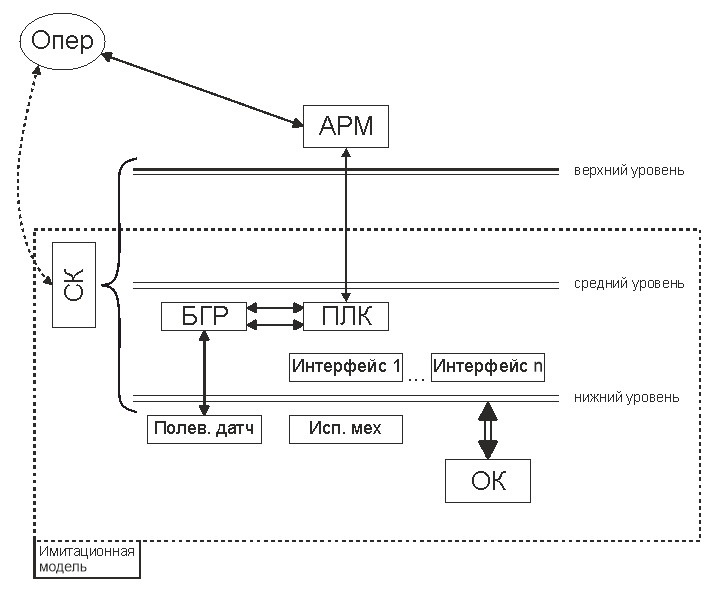
\includegraphics[height=.8\textheight,keepaspectratio]{scheme_3levels.png}\end{center}
\end{frame}



\section{Декомпозиция АНПА}
\begin{frame}{Материальная составляющая модели АНПА}{Выявление общесистемных сущностей}
    \begin{center}
    {\huge Объекты --- Функции --- Действия}\vspace{10mm}
    
    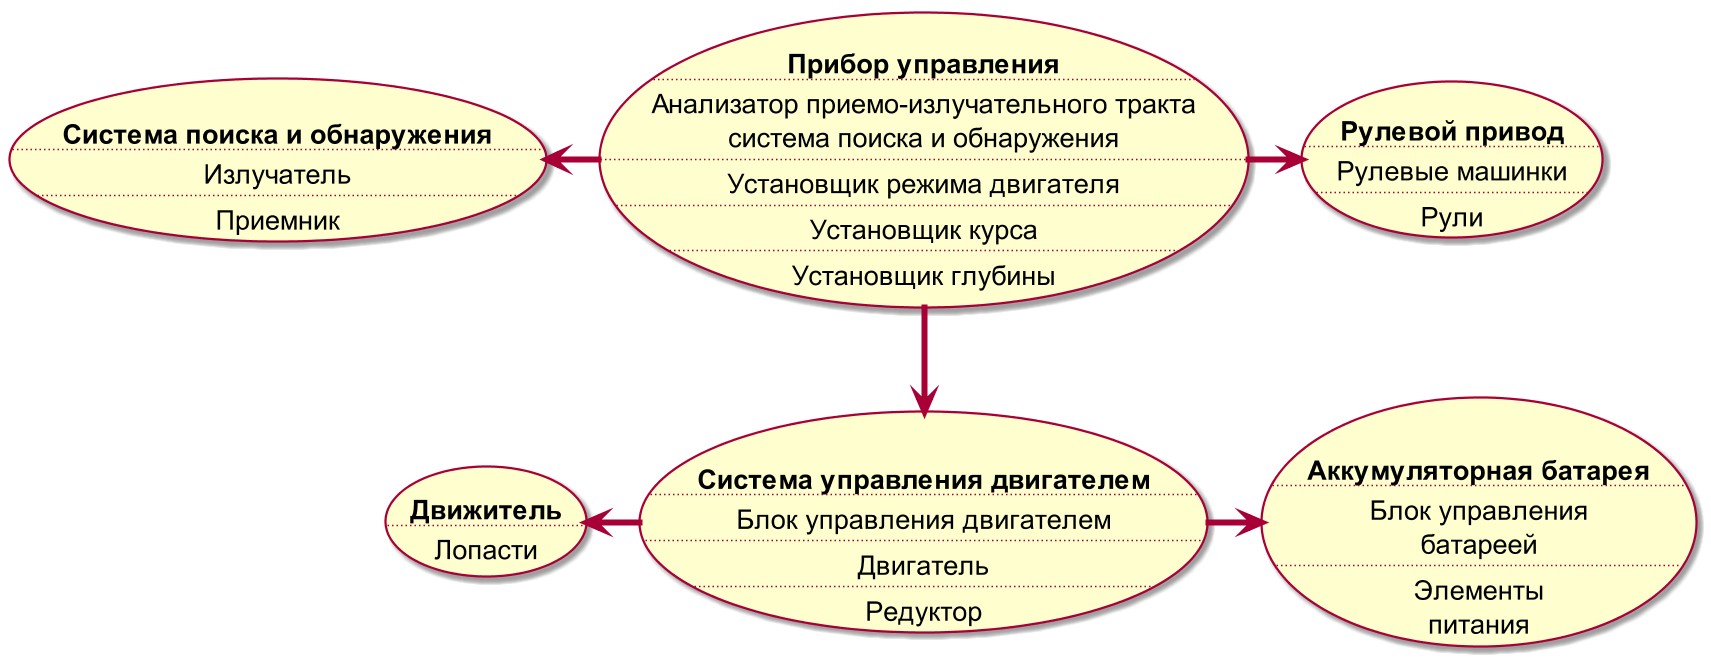
\includegraphics[width=1\linewidth,keepaspectratio]{model_anpa}\vspace{5mm}

    {\color{blue}{\noindent\tiny Елизарова, Н. Применение графоаналитического метода анализа предметной
        области при проектировании информационных систем [Текст] /
        Н. Елизарова, Е. Архангельская // Вестник ИГЭУ. — 2010 — Т. 4 — С. 5 }}

    \end{center}
\end{frame}
\note{
    Отвечаю на вопрос, а какие параметры необходимо имитировать в первую очередь --- \textbf{общесистемные}.
}

\begin{frame}{Объект -- Функция -- Действие}{\small Графоаналитический метод для выявления общесистемных сущностей.}
    {\tiny Елизарова, Н. Применение графоаналитического метода анализа предметной
    области при проектировании информационных систем [Текст] /
    Н. Елизарова, Е. Архангельская // Вестник ИГЭУ. — 2010 — Т. 4 — С. 5 }
    \tiny\begin{tabular}{cp{.2\textwidth}||c|p{.15\textwidth}||cp{.15\textwidth}}
        \toprule
        \multicolumn{2}{|c||}{\textbf{Объект}} & \multicolumn{2}{c||}{\textbf{Функции}} & \multicolumn{2}{c|}{\textbf{Действия}} \\ \midrule
        %
        \multicolumn{1}{|l|}{\multirow{2}{*}{СПО}} & Излучатель                                  & \multirow{5}{*}{Движение}          & Вперед                           & \multicolumn{1}{l|}{\multirow{3}{*}{ПУ}}  & \multicolumn{1}{l|}{Пеленгация целей}     \\ \cline{2-2} \cline{4-4} \cline{6-6}
        \multicolumn{1}{|l|}{}                     & Приемник                                    &                                    & Вправо                           & \multicolumn{1}{l|}{}                     & \multicolumn{1}{l|}{Коррекция курса}      \\ \cline{1-2} \cline{4-4} \cline{6-6}
        \multicolumn{1}{|l|}{\multirow{4}{*}{ПУ}}  & Анализатор приемо-излучательного тракта СПО &                                    & Влево                            & \multicolumn{1}{l|}{}                     & \multicolumn{1}{l|}{Коррекция глубины}    \\ \cline{2-2} \cline{4-4} \cline{5-6}
        \multicolumn{1}{|l|}{}                     & Установщик режима двигателя                 &                                    & Вверх                            & \multicolumn{1}{l|}{\multirow{2}{*}{АКБ}} & \multicolumn{1}{l|}{Хранение}             \\ \cline{2-2} \cline{4-4} \cline{6-6}
        \multicolumn{1}{|l|}{}                     & Установщик курса                            &                                    & Вниз                             & \multicolumn{1}{l|}{}                     & \multicolumn{1}{l|}{Доставка}             \\ \cline{2-6}
        \multicolumn{1}{|l|}{}                     & Установщик глубины                          & \multirow{5}{*}{Питание}           & СПО                              & \multicolumn{1}{l|}{Д}                    & \multicolumn{1}{l|}{Толкает водную среду} \\ \cline{1-2} \cline{4-6}
        \multicolumn{1}{|l|}{\multirow{3}{*}{СУД}} & БУД                                         &                                    & ПУ                               &                                           &                                           \\ \cline{2-2} \cline{4-4}
        \multicolumn{1}{|l|}{}                     & Двигатель                                   &                                    & СУД                              &                                           &                                           \\ \cline{2-2} \cline{4-4}
        \multicolumn{1}{|l|}{}                     & Редуктор                                    &                                    & РП                               &                                           &                                           \\ \cline{1-2} \cline{4-4}
        \multicolumn{1}{|l|}{\multirow{2}{*}{РП}}  & РМ                                          &                                    & Д                                &                                           &                                           \\ \cline{2-4}
        \multicolumn{1}{|l|}{}                     & Рули                                        & \multirow{2}{*}{Обнаружение}       & Излучение зондирующей посылки    &                                           &                                           \\ \cline{1-2} \cline{4-4}
        \multicolumn{1}{|l|}{Д}                    & Лопасти                                     &                                    & Прием отраженого сигнала         &                                           &                                           \\ \cline{1-4}
        \multicolumn{1}{|l|}{\multirow{2}{*}{АКБ}} & БУБ                                         & \multirow{4}{*}{Принятие решений}  & Изменить скорость движения       &                                           &                                           \\ \cline{2-2} \cline{4-4}
        \multicolumn{1}{|l|}{}                     & Модули питания                              &                                    & Изменить курс                    &                                           &                                           \\ \cline{1-2} \cline{4-4}
                                                   &                                             &                                    & Изменить глубину хода            &                                           &                                           \\ \cline{4-4}
                                                   &                                             &                                    & Изменить тип зондирующей посылки &                                           &                                           \\ \cline{3-4}
    \end{tabular}
        \begin{minipage}[t]{0.4\linewidth}
            \centering
                Матрицы связности: 
                \begin{itemize}
                    \item[$A$] взаимосвязь \textbf{Объект -- Функция} 
                    \item[$B$] взаимосвязь \textbf{Функция -- Действие} 
                    \item[$C_1 = A \times B$] взаимосвязь \textbf{Объект -- Действие} 
                \end{itemize}
        \end{minipage}
        \hfill
        \begin{minipage}[t]{0.55\linewidth}
            \vspace{1pt} $C_2 = \begin{pmatrix} \sum_{j=1}^l c_{1\,1j} \\ \ldots \\ \sum_{j=1}^l c_{1\,mj} \\ \end{pmatrix}\!; \quad C_3 = \left. \frac{C_2}{l} \right|_{l \equiv 6}$
        \end{minipage}
\end{frame}
    
\begin{frame}
    \tiny
    \begin{equation*}
        \begin{split}
        A_{16\times14} = &\begin{pmatrix}
            0 & 0 & 0 & 0 & 0 & 1 & 0 & 0 & 0 & 0 & 1 & 0 & 0 & 0 & 0 & 0 \\
            0 & 0 & 0 & 0 & 0 & 1 & 0 & 0 & 0 & 0 & 0 & 1 & 0 & 0 & 0 & 0 \\
            0 & 0 & 0 & 0 & 0 & 1 & 1 & 0 & 0 & 0 & 0 & 1 & 0 & 0 & 0 & 1 \\
            0 & 0 & 0 & 0 & 0 & 0 & 0 & 1 & 0 & 1 & 0 & 0 & 0 & 0 & 0 & 0 \\
            0 & 1 & 1 & 0 & 0 & 0 & 0 & 0 & 0 & 0 & 1 & 0 & 0 & 1 & 0 & 1 \\
            0 & 0 & 0 & 1 & 1 & 0 & 0 & 0 & 0 & 0 & 0 & 0 & 0 & 0 & 1 & 0 \\
            0 & 0 & 0 & 0 & 0 & 1 & 0 & 0 & 0 & 0 & 0 & 0 & 1 & 0 & 0 & 0 \\
            0 & 0 & 0 & 0 & 0 & 1 & 0 & 0 & 0 & 0 & 0 & 0 & 1 & 0 & 0 & 0 \\
            0 & 0 & 0 & 0 & 0 & 0 & 0 & 0 & 0 & 1 & 0 & 0 & 0 & 0 & 0 & 0 \\
            1 & 1 & 1 & 1 & 1 & 0 & 0 & 0 & 0 & 0 & 0 & 0 & 0 & 1 & 1 & 0 \\
            1 & 1 & 1 & 1 & 1 & 0 & 0 & 0 & 0 & 0 & 0 & 0 & 0 & 1 & 1 & 0 \\
            0 & 0 & 0 & 0 & 0 & 0 & 0 & 0 & 0 & 0 & 0 & 0 & 0 & 1 & 1 & 0 \\
            0 & 0 & 0 & 0 & 0 & 1 & 1 & 1 & 1 & 1 & 1 & 0 & 0 & 0 & 0 & 0 \\
            0 & 0 & 0 & 0 & 0 & 0 & 0 & 0 & 0 & 0 & 1 & 1 & 0 & 0 & 0 & 0 \\
        \end{pmatrix},{}\\
    %
        B_{6\times16} = &\begin{pmatrix}
            0 & 0 & 0 & 0 & 0 & 0 & 0 & 0 & 0 & 0 & 1 & 1 & 0 & 0 & 0 & 1 \\
            0 & 1 & 1 & 0 & 0 & 0 & 0 & 0 & 0 & 0 & 0 & 1 & 1 & 1 & 0 & 0 \\
            0 & 0 & 0 & 1 & 1 & 0 & 0 & 0 & 0 & 0 & 0 & 0 & 1 & 0 & 1 & 0 \\
            0 & 0 & 0 & 0 & 0 & 1 & 1 & 1 & 1 & 1 & 0 & 0 & 0 & 0 & 0 & 0 \\
            0 & 0 & 0 & 0 & 0 & 1 & 1 & 1 & 1 & 1 & 1 & 0 & 0 & 0 & 0 & 1 \\
            1 & 0 & 0 & 0 & 0 & 0 & 0 & 0 & 0 & 0 & 0 & 0 & 1 & 1 & 1 & 0 \\
        \end{pmatrix}^T\,,{}\\
    %
        C_1 = A \times B = &\begin{pmatrix}
            1 & 1 & 2 & 0 & 2 & 0 & 0 & 0 & 0 & 0 & 0 & 0 & 1 & 2 \\
            0 & 1 & 1 & 0 & 3 & 0 & 1 & 1 & 0 & 3 & 3 & 1 & 0 & 1 \\
            0 & 0 & 0 & 0 & 0 & 3 & 1 & 1 & 0 & 3 & 3 & 1 & 0 & 0 \\
            1 & 1 & 2 & 2 & 0 & 0 & 1 & 1 & 1 & 0 & 0 & 0 & 5 & 0 \\
            2 & 1 & 3 & 2 & 2 & 0 & 1 & 1 & 1 & 0 & 0 & 0 & 6 & 1 \\
            0 & 0 & 0 & 0 & 1 & 1 & 1 & 1 & 0 & 3 & 3 & 2 & 0 & 0 \\
        \end{pmatrix}^T_{6\times14}\,,{}\\
    %
        C_3 = &\left. \frac{C_2}{l} \right|_{l \equiv 6} = 
            \left( 0.67\;\; 0.67\;\; \textbf{1.33}\;\; 0.67\;\; \textbf{1.33}\;\; 0.67\;\; 0.83\;\; 0.83\;\; 
            0.33\;\; \textbf{1.50}\;\;\textbf{1.50}\;\; 0.67\;\; \textbf{2.00}\;\; 0.67 \right)^T\,.
    \end{split}
    \end{equation*} 

    Пороговое значение $K_{min} = \overline{C_3} = 0.98$
    \begin{itemize}
        \item[2.0]   блок управления батареей;
        \item[1.5]   рулевые машинки, рулевой привод;
        \item [1.33] анализатор приемо-излучательного тракта СПО и установщик курса.
    \end{itemize}
\end{frame}




\section{Таксономия классов}
\subsection{Графики зависимости}
\begin{frame}{Временные зависимости}{Захват значения}
    \vspace{-20mm}
    \begin{minipage}[c]{0.47\linewidth}
        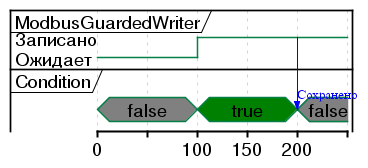
\includegraphics[width=1\linewidth]{modbus_guarded_writer}%
        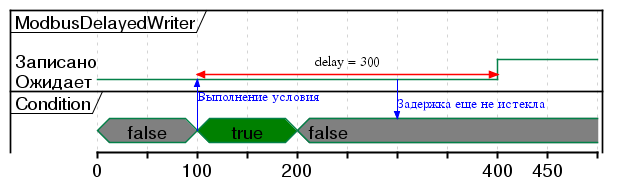
\includegraphics[width=1\linewidth]{modbus_delayed_writer}
    \end{minipage}

    \begin{minipage}[c]{0.47\linewidth}
        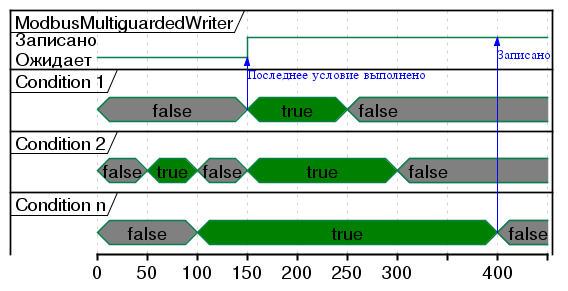
\includegraphics[width=1\linewidth]{modbus_multiguarded_writer.png}%
        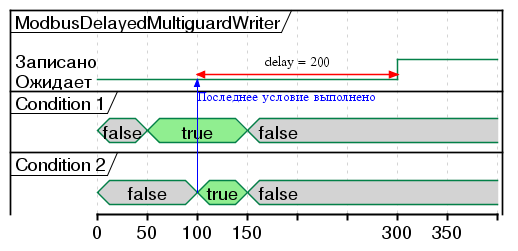
\includegraphics[width=1\linewidth]{modbus_delayed_multiguarded_writer.png}
    \end{minipage}
\end{frame}
\begin{frame}{Временные зависимости}{Захват значения}
    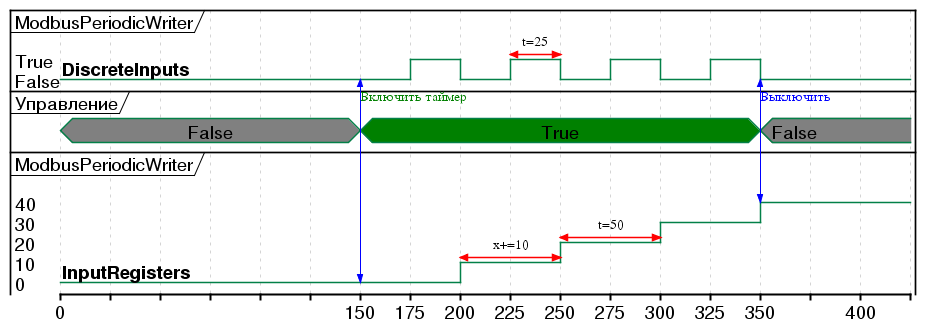
\includegraphics[width=1\linewidth]{modbus_periodic_writer.png}
\end{frame}


\subsubsection{Перегрузка методов}
\begin{frame}{Полимофизм}{Перегрузка методов}
    \hspace{-10mm}\begin{table}
        \begin{center}
        \begin{tabular}{|l|c|c|c|c|c|c||c|c|}
        \hline
            \multicolumn{1}{|c|}{\multirow{2}{*}{Наследники}} &
            \multicolumn{6}{c||}{\textbf{атрибуты}} &
            \multicolumn{2}{c|}{\textbf{override}} \\ \cline{2-9} %Переопределенные методы наследника
            \multicolumn{1}{|c|}{}     &
                \rotatebox{90}{tag} & \rotatebox{90}{value}  & \rotatebox{90}{delay}  & \rotatebox{90}{period} &
                \rotatebox{90}{delta} & \rotatebox{90}{duration} &
                \rotatebox{90}{conditionsMet} & \rotatebox{90}{newModbusData} \\ \hline
            {\tiny\texttt{ModbusGuardedWriter}}              & +    & +      & -      & -      & - &-     & + & -  \\ \hline
            {\tiny\texttt{ModbusMultiguardedWriter}}         & +    & +      & -      & -      & - &-     & + & -  \\ \hline
            {\tiny\texttt{ModbusDelayedWriter}}              & +    & +      & +      & -      & - &-     & - & +  \\ \hline
            {\tiny\texttt{ModbusDelayedMultiguardWriter}}    & +    & +      & +      & -      & - &-     & - & +  \\ \hline
            {\tiny\texttt{ModbusPeriodicWriter}}             & +    & +      & -      & +      & + &$\pm$ & + & -  \\ \hline
        \end{tabular}
        \end{center}
    \end{table}
\end{frame}


\subsection{Работа составных частей имитатора}
\begin{frame}{Жизненный цикл}
    \begin{center}
        \includegraphics<1>[width=1\linewidth]{modbus_class_components.png}
        \includegraphics<2>[height=.8\textheight]{top_level.png}
        \includegraphics<3>[height=.8\textheight]{modbuselementwriterimpl}
    \end{center}
\end{frame}


\begin{frame}{Жизненный цикл интерфейса \texttt{IModbusElementWriter}}
    \begin{center}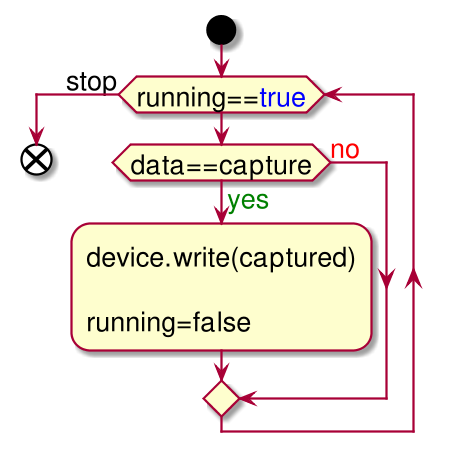
\includegraphics[height=.8\textheight]{imodbuselementwriter_activity.png}\end{center}
\end{frame}

\section{Листинги}\subsection{XML}
\begin{frame}{XML}{Мгновенная запись}
    \lstinputlisting[language=MyXML,basicstyle=\tiny]{Dissertation/listings/xml/guarded.xml}
\end{frame}
\begin{frame}{XML}{Множественные условия}
    \lstinputlisting[language=MyXML,basicstyle=\tiny]{Dissertation/listings/xml/multiguarded.xml}
\end{frame}
\begin{frame}{XML}{Запись с задержкой}
    \lstinputlisting[language=MyXML,basicstyle=\tiny]{Dissertation/listings/xml/delayed.xml}
\end{frame}
\begin{frame}{XML}{Периодическая запись}
    \lstinputlisting[language=MyXML,basicstyle=\tiny]{Dissertation/listings/xml/periodic.xml}
\end{frame}


\section{Онтология}
\subsection{Классы}
\begin{frame}{Онтология}
    \begin{center}
    \includegraphics<1>[width=.9\textwidth,keepaspectratio]{owl/anpa_hierarchy.png}
    \includegraphics<2>[width=.9\textwidth,keepaspectratio]{owl/part_of.png}
    \includegraphics<3>[width=.9\textwidth,keepaspectratio]{owl/function_movement.png}
    \end{center}
\end{frame}

\subsection{SPARQL}
\begin{frame}[fragile]{Пример SPARQL запроса}{Получение новых знаний}
    \begin{lstlisting}[language=sparql]
PREFIX anpa:<http://.../guap/ontologies/z8430m/ANPA#>
SELECT ?volt ?condition ?delay ?newvalue 
       ?relation ?condvalue ?title
WHERE { ?volt anpa:ИмеетУсловие ?condition .
    ?volt anpa:value ?newvalue .
    ?condition anpa:relation ?relation .
    ?condition anpa:title ?title .
    ?condition anpa:value ?condvalue .
    ?volt anpa:delay ?delay . FILTER (?delay > 100) . }
    \end{lstlisting}\vspace{-5mm}
    
    \begin{table}
        \begin{center}
            \begin{tabular}{cl}\hline
                volt & Uv\_пу \\\hline
                condition & C1 \\\hline
                delay & 500 \\\hline
                newvalue & 27 \\\hline
                relation & Eq \\\hline
                condvalue & true \\\hline
                title & C1 \\\hline
            \end{tabular}
        \end{center}
    \end{table}
\end{frame}


\section{GUI}
\begin{frame}{GUI}
    \begin{center}
        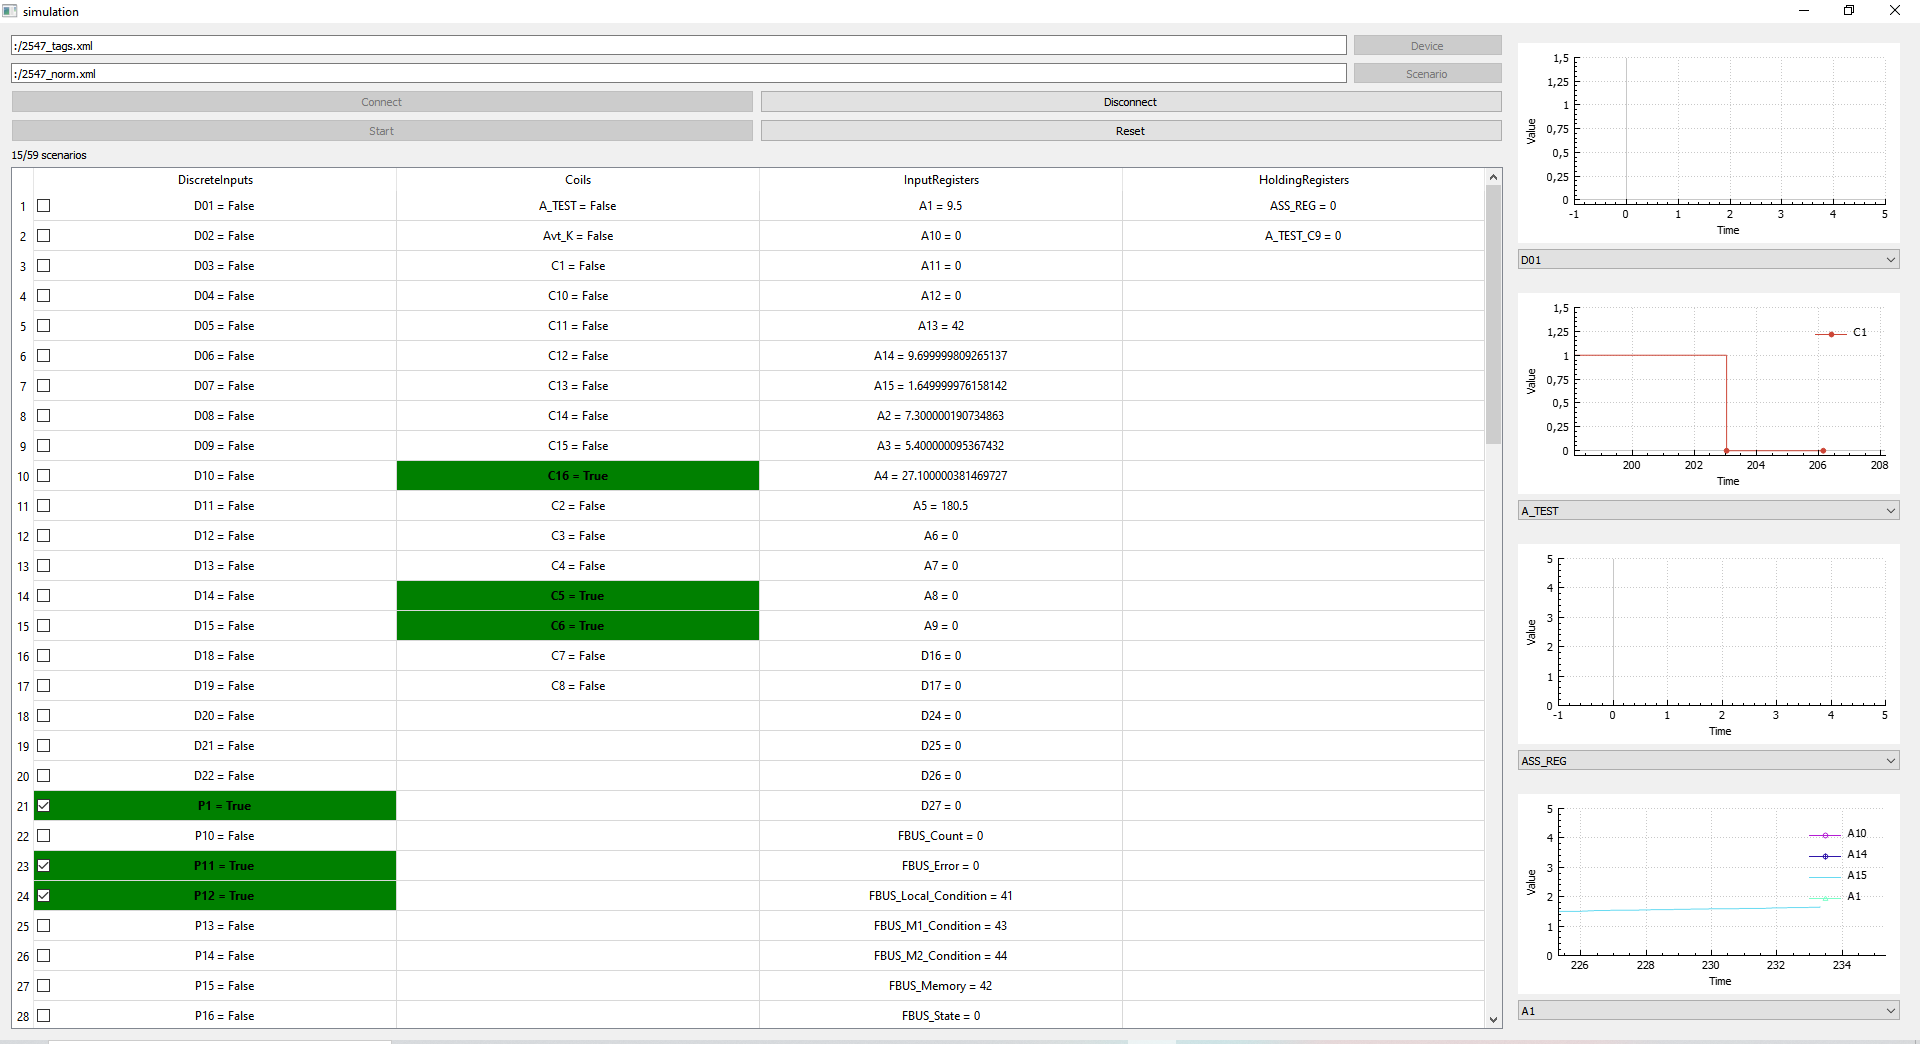
\includegraphics[width=1\linewidth]{imitator.png}
    \end{center}
\end{frame}
